%-----------------------------------LICENSE------------------------------------%
%   This file is part of tikz_figures.                                         %
%                                                                              %
%   tikz_figures is free software: you can redistribute it and/or              %
%   modify it it under the terms of the GNU General Public License as          %
%   published by the Free Software Foundation, either version 3 of the         %
%   License, or (at your option) any later version.                            %
%                                                                              %
%   tikz_figures is distributed in the hope that it will be useful,            %
%   but WITHOUT ANY WARRANTY; without even the implied warranty of             %
%   MERCHANTABILITY or FITNESS FOR A PARTICULAR PURPOSE.  See the              %
%   GNU General Public License for more details.                               %
%                                                                              %
%   You should have received a copy of the GNU General Public License along    %
%   with tikz_figures.  If not, see <https://www.gnu.org/licenses/>.           %
%------------------------------------------------------------------------------%

% Use the standalone class for displaying the tikz image on a small PDF.
\documentclass[crop, tikz]{standalone}

% Import the tikz and pgfplots packages to use for the drawing.
\usepackage{tikz, pgfplots}

% Begin the document.
\begin{document}

    % Draw the figure.
    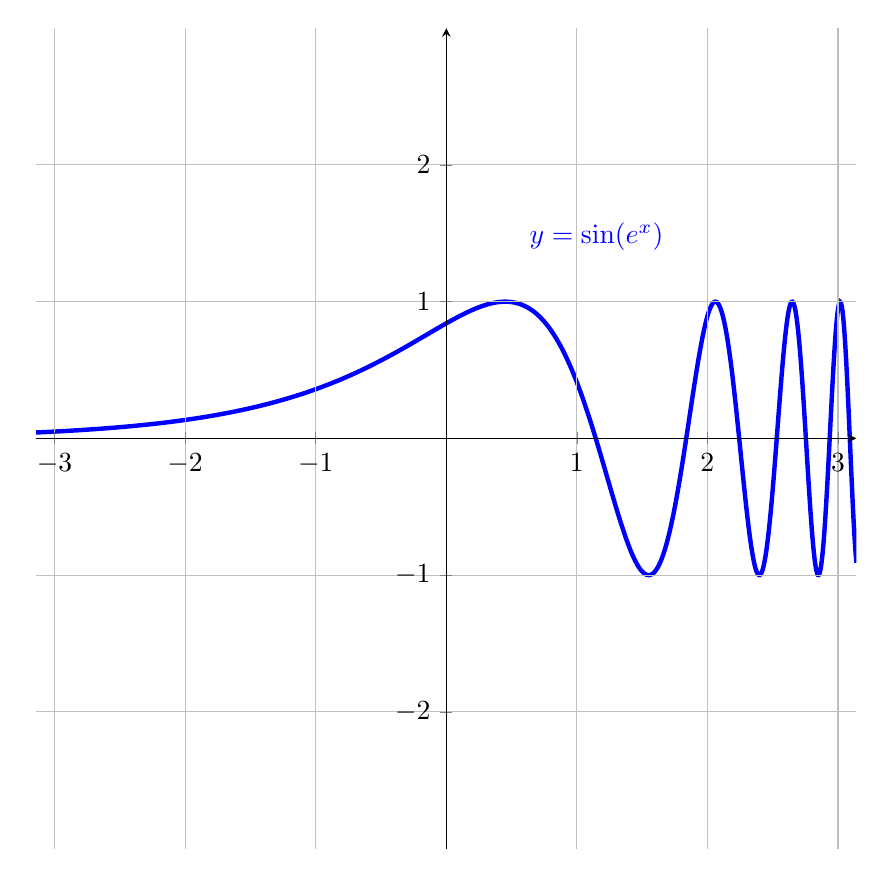
\begin{tikzpicture}
        \begin{axis}[
            axis y line = center,
            axis x line = middle, 
            axis on top = true,
            xmin = -pi,
            xmax = pi,
            ymin = -3,
            ymax = 3,
            height = 12.0cm,
            width = 12.0cm,
            grid,
            xtick = {-5, ..., 5},
            ytick = {-2, -1, ..., 2},
            restrict y to domain = -3:3
        ]

            % pgfplots provides a plotting routines.
            \addplot [%
                domain = -pi:pi,
                samples = 1000,
                mark = none,
                ultra thick,
                blue
            ] {sin(deg(e^(x)))};

            % Label the plot.
            \node [above, blue] at (axis cs: 1.15,1.3) {$y=\sin(e^{x})$};
        \end{axis}
    \end{tikzpicture}
\end{document}
